\documentclass[a4paper,12pt]{scrartcl}
\usepackage[margin=2.5cm
  %,showframe% <- only to show the page layout
  ]{geometry} % change margin to more compact
%%%%%% header matter %%%%%%
\usepackage[T1]{fontenc}
\usepackage{enumitem}
\usepackage{amsmath}
\usepackage{graphicx}
\usepackage{float}
\usepackage{xcolor}
\usepackage{authblk} % Allows for authors from multiiple institutes
\usepackage{siunitx} % Allow for scientific unit
\usepackage{hyperref}
\hypersetup{colorlinks,%
            citecolor=black,%
            filecolor=black,%
            linkcolor=black,% link like content or so
            urlcolor=blue,%
            pdftex}
\usepackage{lineno} % to use \linenumbers
\linenumbers % give line number as a draft version
%%%%%% start: code style %%%%%%

\usepackage{listings}
%\usepackage{color}
\definecolor{codegreen}{rgb}{0,0.6,0}
\definecolor{codegray}{rgb}{0.5,0.5,0.5}
\definecolor{codepurple}{rgb}{0.58,0,0.82}
\definecolor{backcolour}{rgb}{0.95,0.95,0.92}

\lstdefinestyle{mystyle}{
    backgroundcolor=\color{backcolour},
    commentstyle=\color{codegreen},
    keywordstyle=\color{magenta},
    numberstyle=\tiny\color{codegray},
    stringstyle=\color{codepurple},
    basicstyle=\footnotesize\ttfamily,
    columns=fullflexible,
    breakatwhitespace=false,
    breaklines=true,
    captionpos=b,
    keepspaces=true,
    numbers=left,
    numbersep=5pt,
    showspaces=false,
    showstringspaces=false,
    showtabs=false,
    tabsize=2,
    belowskip=0.05em
}

\lstset{style=mystyle}
%%%%%% end: code style %%%%%%

%%%%%% header matter %%%%%%

\title{
\includegraphics[width=10cm]{figs/DESYTestBeam.png}  
\includegraphics[width=10cm]{figs/Aida2020.png} \\ \vspace{2cm} USER MANUAL \\ Slow Control System}
\author[*]{Lars Fischer}
\author[*]{Mengqing Wu}
\affil[*]{Deutsches Elektronen-Synchrotron DESY, Notkestr. 85, 22607 Hamburg, Germany}

\date{\today}

\begin{document}
\clearpage\maketitle
This document serves as a how-to manual for the common environmental Slow Control System at DESY test beam facility. This system is has a rack-based hardware, connecting to the test beam common DAQ, EUDAQ2, via a SQL DataBase, MySQL.
Its hardware and software will be introduced briefly, with a focus on the following concepts:
a step-by-step instruction of the installation and the configuration of the software;
a easy-to-follow guide for users who wish to integrate their own slow control inputs to our system, or to the common EUDAQ2 datastream.
\thispagestyle{empty}
\cleardoublepage

\tableofcontents
\pagebreak

\section{Introduction}
\subsection{Hardware and software}
The Slow Control System is currently able to collect connected sensor data in a configurable frequence (i.e. how frequent to update the DataBase variables from sensor data), transfer to the test beam common DAQ, EUDAQ2, and finally write to user data taking events as a standard EUDAQ raw event tag, i.e. not affecting any user customized event definition.
For further reading, a detailed description of the system design and a manual for developers, please see the following documents:
\begin{itemize}
  \item Deliverable Report: \href{https://cds.cern.ch/record/2290758/files/AIDA-2020-D15\_3.3.pdf}{\footnotesize{https://cds.cern.ch/record/2290758/files/AIDA-2020-D15\_3.3.pdf}};
  \item Main User Manual: \href{https://cds.cern.ch/record/2284369/files/AIDA-2020-NOTE-2017-007.pdf}{\footnotesize{https://cds.cern.ch/record/2284369/files/AIDA-2020-NOTE-2017-007.pdf}}.
\end{itemize}
This document will guide you step by step through the software design and all necessary installations.


\subsubsection*{Rack and sensors}
The DAQ system hardware is a rack-based system which is movable and connected via an Ethernet cable, as shown in Figure~\ref{fig:sc-rack}; it is currently equipped with \textbf{10 NTC sensors} for temperature measurements in an operation range of \SI{-20}{\celsius} to \SI{+100}{celsius} \footnote{NB: to be confirmed, not sure where Lars found this info...}, and \textbf{one DIGI sensor} for complimentary measurements of air pressure, dew point and humidity.
\begin{figure}[!ht]
  \centering
  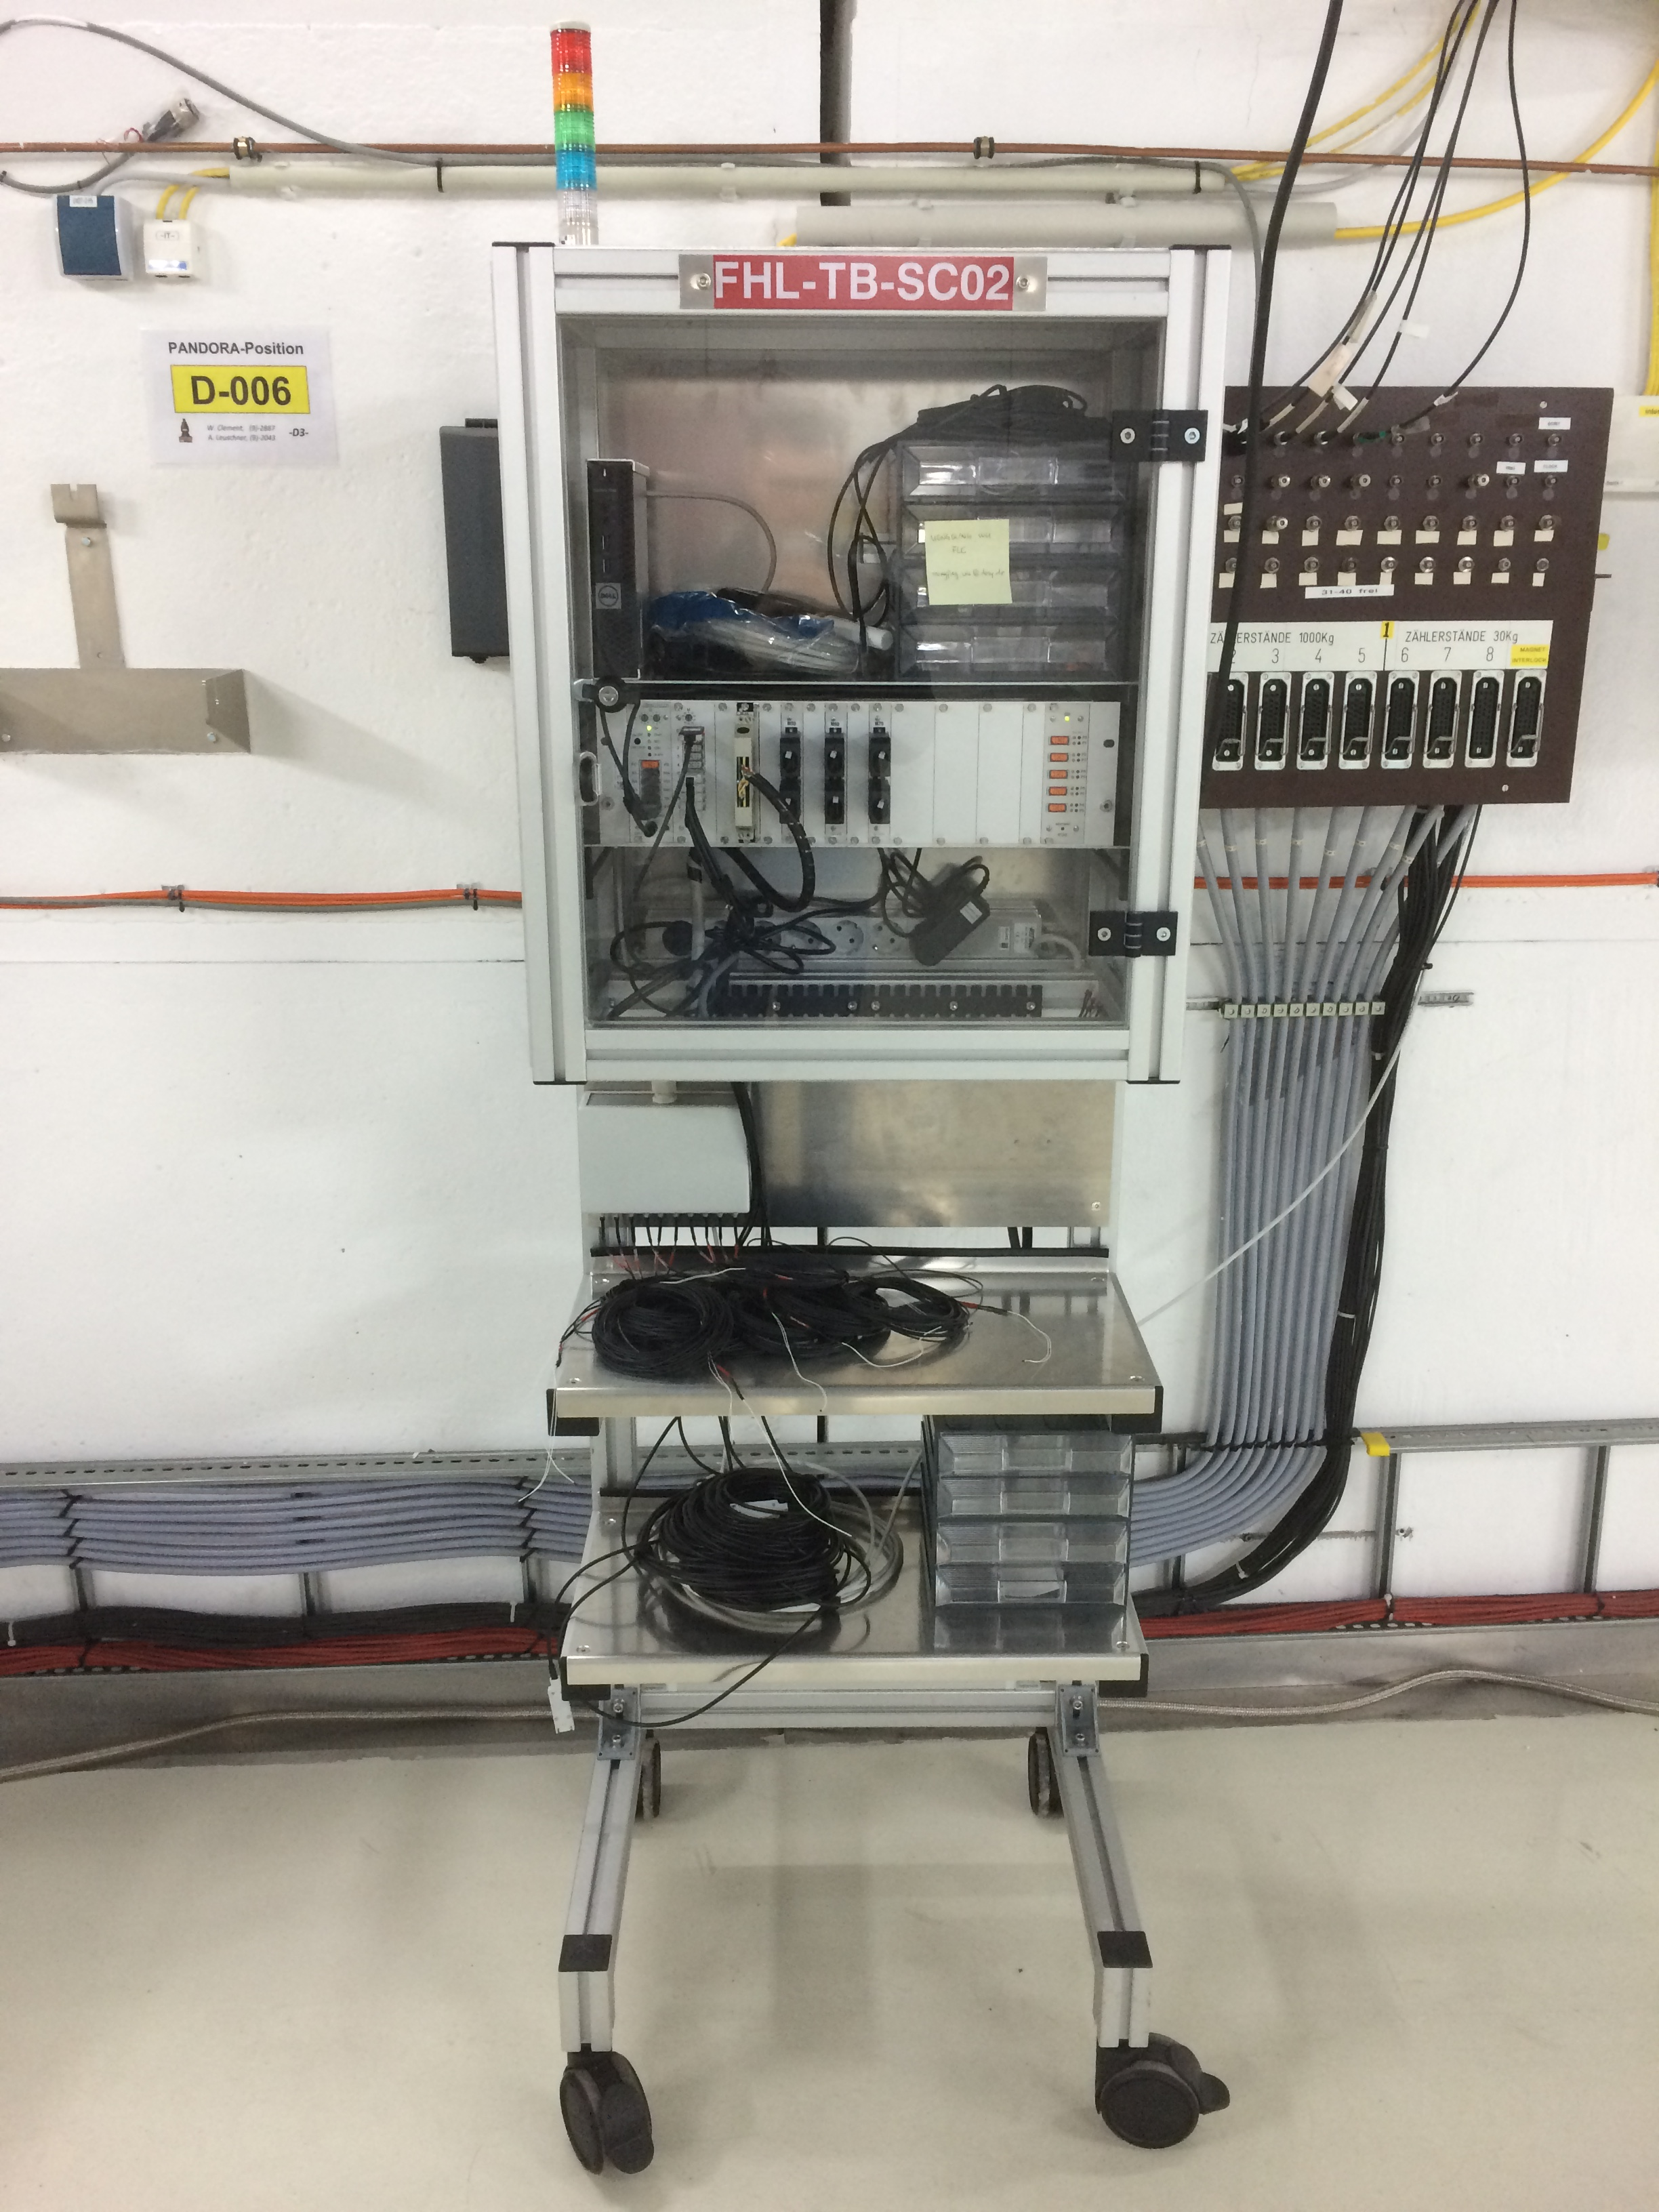
\includegraphics[height=7cm]{figs/Rackganz.jpg}%
  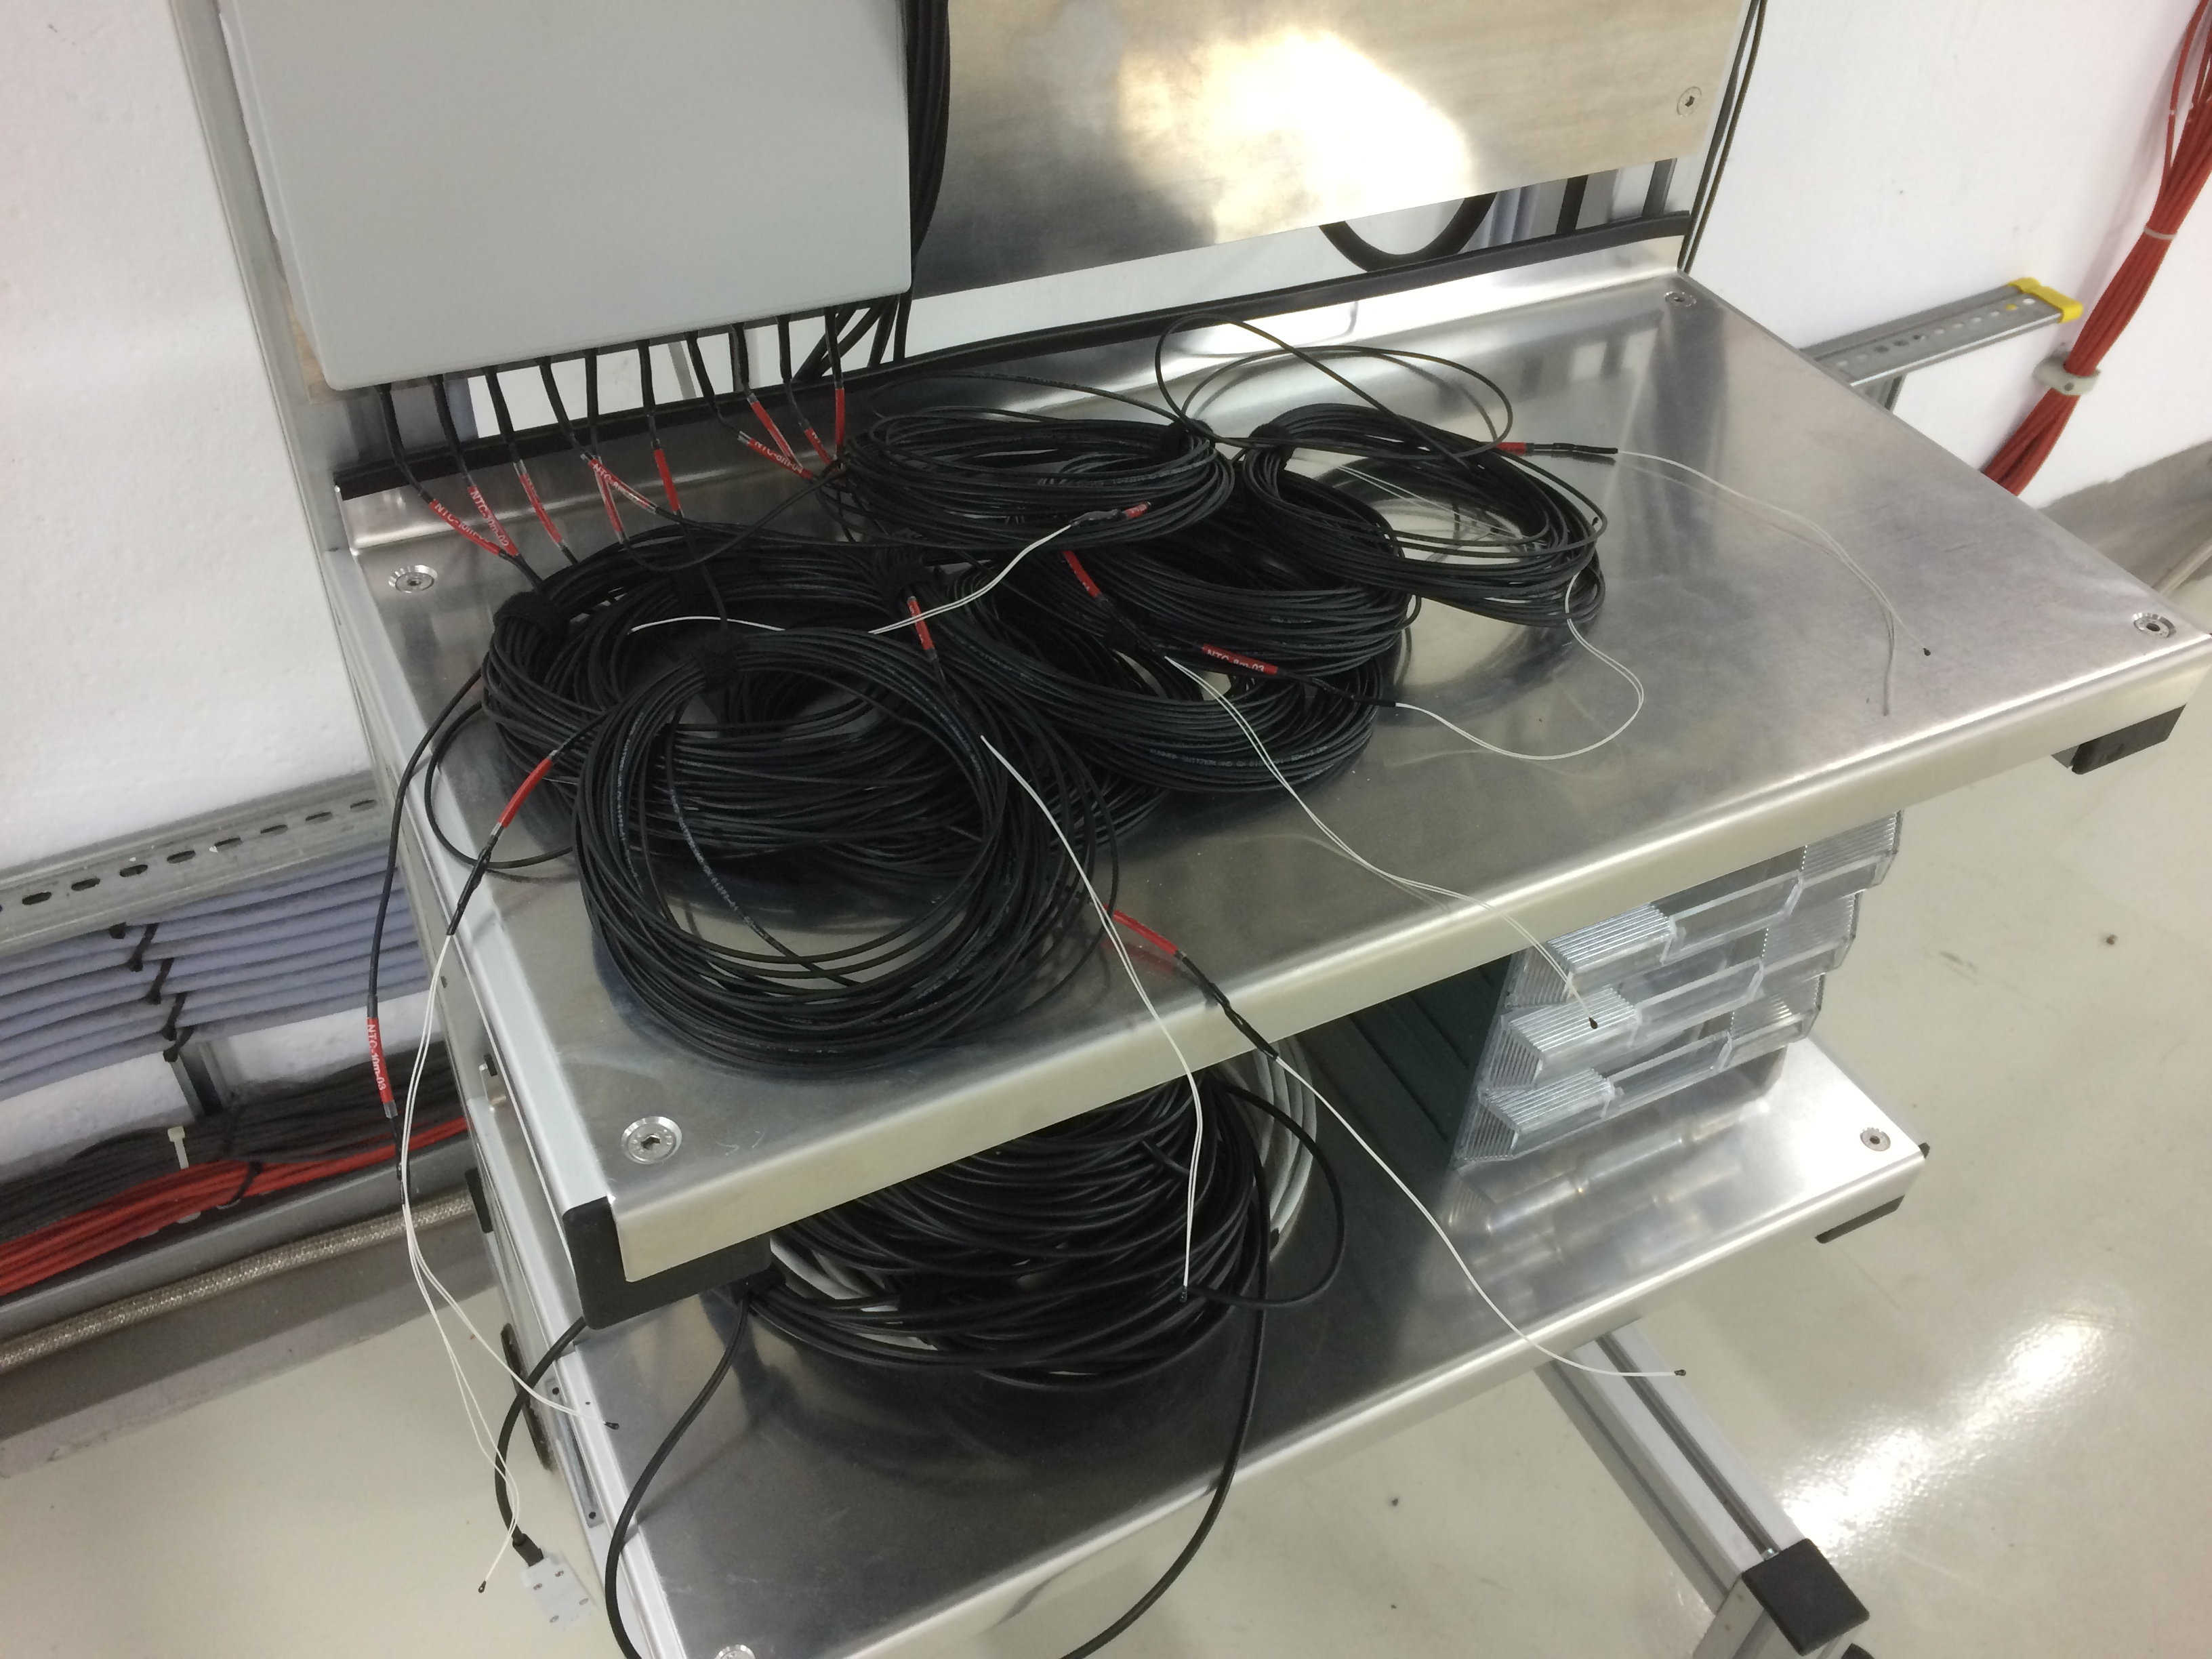
\includegraphics[height=7cm]{figs/Sensoren.jpg}
\caption{Slow Control System rack \#02 (left) in DESY test beam area TB24 and the 10 NTC sensors of \SI{10}{m} long (right).}
\label{fig:sc-rack}
\end{figure}

The NTC sensors are \SI{10}{m} long that can be located at different measuring points in a beam area, according to user needs; the DIGI sensor is fixed at the rear of the rack, and can be used as alarm monitor~\footnote{There is \textbf{a LED-based alarm} available on the rack (seated on the top of the rack), however, it is not yet plugged to test; users are also able to use it with their defined warning signals.}. All the sensors are connected to a data logger (ALMEMO) via a special connector. Users are also able to \textbf{mount their own sensors} to the data collector, with many spared connectors stored on the rack, but \textbf{please contact the local support team before any customized modification to the system!}

\subsubsection*{Software}
The DAQ software consists of \textbf{a commercial DAQ (AMR)} and a testbeam common DAQ software, \textbf{EUDAQ2}.
The data logger is connected to a Windows-PC mounted on the rack, and it is polled via a USB connector by a commercial DAQ software (AMR) provided by the same company.

This document will give a detailed instruction to guide you to configure and to use the DAQ system to get a measurement based on the connected sensors.

\subsection{Status and Note for usage}
The DESY test beam facility includes three beam areas, TB21, TB22, with TB24 and TB24/1 in tandem as shown in Figure~\ref{fig:desytb}. \textbf{Two} Slow Control racks are currently available to move around at the test beam for different use cases.

\begin{figure}[!ht]
  \centering
  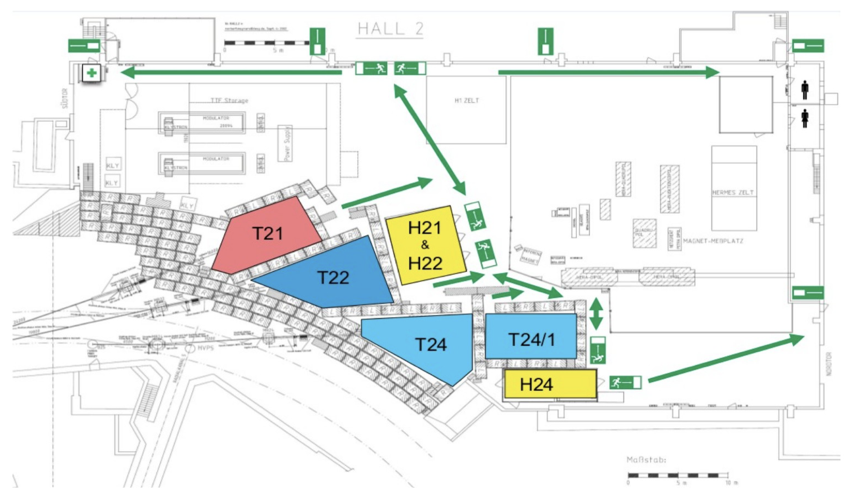
\includegraphics[width=0.8\textwidth]{figs/Testbeam.png}
\caption{Slow Control System Racks can be moved in T21/T22/T24 for observing.}
\label{fig:desytb}
\end{figure}

The power and Internet connection should always be connected, while the Slow Control System is in use. Once the power was off, in order to continue the slow control data streaming, one needs to: 1) release the beam area interlock; 2) check to ensure the data logger is on, and the PC is on.

You can of course do the following things, however, please kindly inform the contact person \textbf{before}:
\begin{itemize}
  \item disconnect the Ethernet cable and/or unpower the slow control system;
  \item replace the NTC sensors;
  \item relocate the rack by rolling it among different test beam areas or even to other work space;
\end{itemize}

\section{DAQ architecture}
\subsection{Structure}
The system data acquisition (DAQ) is implemented by two PCs running in parallel, see Figure~\ref{fig:DAQflow}.
The DAQ is developped based on the current hardware, that user only needs to: 1) load a testbeam slow control \textit{Producer} module in EUDAQ2 as you will do to load your device; 2) copy/paste the prepared slow control config file to your config file; 3) run the EUDAQ2 like how you will do to take data from your device. At the end of the run, once all the data is written to a standard EUDAQ2 raw file, you can find all the slow control data recorded as tags in your event.

\begin{figure}[!ht] \centering
%\includegraphics[trim={5cm .5cm 2cm 5cm},clip,width=\textwidth]{FlowChartSCS.png}
\includegraphics[width=0.85\textwidth]{figs/FlowChartSCS.png}
\caption{Flow chart of the Slow Control System}
\label{fig:DAQflow}
\end{figure}

\subsection{Windows Rack PC}
The Windows PC on the rack collects the data from data logger (ALMEMO) with a commercial DAQ software (AMR).
With a default (updated in Jan 2018) configuration: AMR software polls data from data logger every \SI{30}{s}.
An ODBC is set up to forward the values into a MySQL (version 5.7.20) based database on the Linux-PC.

\subsection{Linux PC}
The ODBC connector shown in Figure~\ref{fig:DAQflow} connects the Windows Operating System (OS) with any remote DataBase (DB) using the DB's TCP/IP address. Therefore, if the internect connection of either of the two PCs is disconnected, no data can be transferred to the User.

A MySQL Database with necessary tables are set on a Linux PC at DESY, in order to transfer all the connected sensor channels; the relevant setup to send data out from the Windows PC is also prepared. As long as the Windows PC starts to Poll and send out data, the relevant tables in the MySQL DataBase will be filled with entries ordered by timestampes, if both PCs are on and connected to the Internet with their IP addresses not changed).

The EUDAQ2 software is installed on this Linux PC, and it reads out entries from the MySQL tables.
A unix-ODBC is installed to connect the MySQL database with the EUDAQ2 framework.
User can use the EUDAQ2 GUI with prepared Producer and Data collector modules loaded via a command line command, and once User start one EUDAQ2 run with all the relevant GUI, the slow control data will be written down to the standard EUDAQ raw event as tags.
%The EUDAQ software collects data in user defined timestamps from the database on the Linux PC.
%While the data is transfered into the database the second DAQ software collects only the events of the timestamps the user adjusted. The EUDAQ can simply be handled by an own GUI.
After data taking the output can be converted from EUDAQ raw/native file into a readable csv file, with a provided command line converter. Furthermore, there are macros provided to plot the csv data.

\section{Software Setup} \label{sec:swsetup}
There are \textbf{two APIs} and \textbf{three softwares} to install and to configure:
\begin{itemize}
  \item API:
  \begin{itemize}
    \item ODBC: 32-bit needed, installed by default in Windows, need to install MySQL driver and configure a DSN for the remote MySQL DB;
    \item unixODBC: installation needed, as well as a MySQL driver~\cite{mysql-odbc} to install and a DSN to add/configure for connection to MySQL DataBase;
  \end{itemize}

  \item Software:
  \begin{itemize}
    \item AMR: installed under purchase on the Windows Rack PC, ODBC DSN entry needed to add/configure for data transmit (Tx);
    \item MySQL: installation needed, needs to add target DataBase with tables to receive (Rx) data sent from AMR;
    \item EUDAQ2: installation needed, modules and configuration prepared for default setup; configurable variables in .conf files, to change DataBase and/or target tables.
  \end{itemize}
\end{itemize}

\subsection{MySQL}
The MySQL database on the Linux PC is the central interaction point of the two DAQ softwares. First of all there has to be a user which can be used from multiple hostes. This is required so that the AMR software on the Windows PC can remotly access the database. Therefore the certain user has to get access privileges from different computers.

\subsubsection*{Installation}

Install the MySQL server by using the Ubuntu package manage:
\begin{lstlisting}[language=bash]
sudo apt-get updated
sudo apt-get install mysql-server
\end{lstlisting}

After the installtion, run the \verb|mysql_secure_installation| utility, with which you can define the MySQL root user password, configure remote access and etc.
It is simple to start the MySQL shell as the root user with the password you just set:
%\colorbox{lightgray}{\texttt{mysql -u username -p}} \\
\begin{lstlisting}[language=SQL]
mysql -u root -p
mysql>
\end{lstlisting}

\subsubsection*{Remote access configuration}
There are \texttt{database}, with \texttt{tables} inside, which are accessable for different \texttt{user}s available at different \texttt{host}s in MySQL.
\begin{itemize}
  \item At least two users needed: one is write-only for the AMR to access the DataBase and the other is read-only for the EUDAQ2.
  \item To maintain database/tables for different machines, one can use:
  \begin{itemize}
    \item either: create one \texttt{database} for each rack, including one unit \texttt{table} and one data receiving \texttt{table};
    \item or: create one \texttt{database} for \textbf{ALL} racks, providing one common unit \texttt{table}, but one data receiving \texttt{table} for each machine.
    \item the current strategy is to have one database for one rack with one unit tabke and one data receiving table provided.
  \end{itemize}
\end{itemize}

\subsubsection*{Useful MySQL Commands}

You can check all the users with the corresponding hosts using the following command:
%\colorbox{lightgray}{\texttt{mysql> SELECT user, host FROM mysql.user;}}\\
\begin{lstlisting}[language=SQL]
mysql> SELECT user, host FROM mysql.user;
\end{lstlisting}

Then you should see an output as shown in Figure~\ref{fig:mysql-user}:
\begin{figure}[!ht] \centering
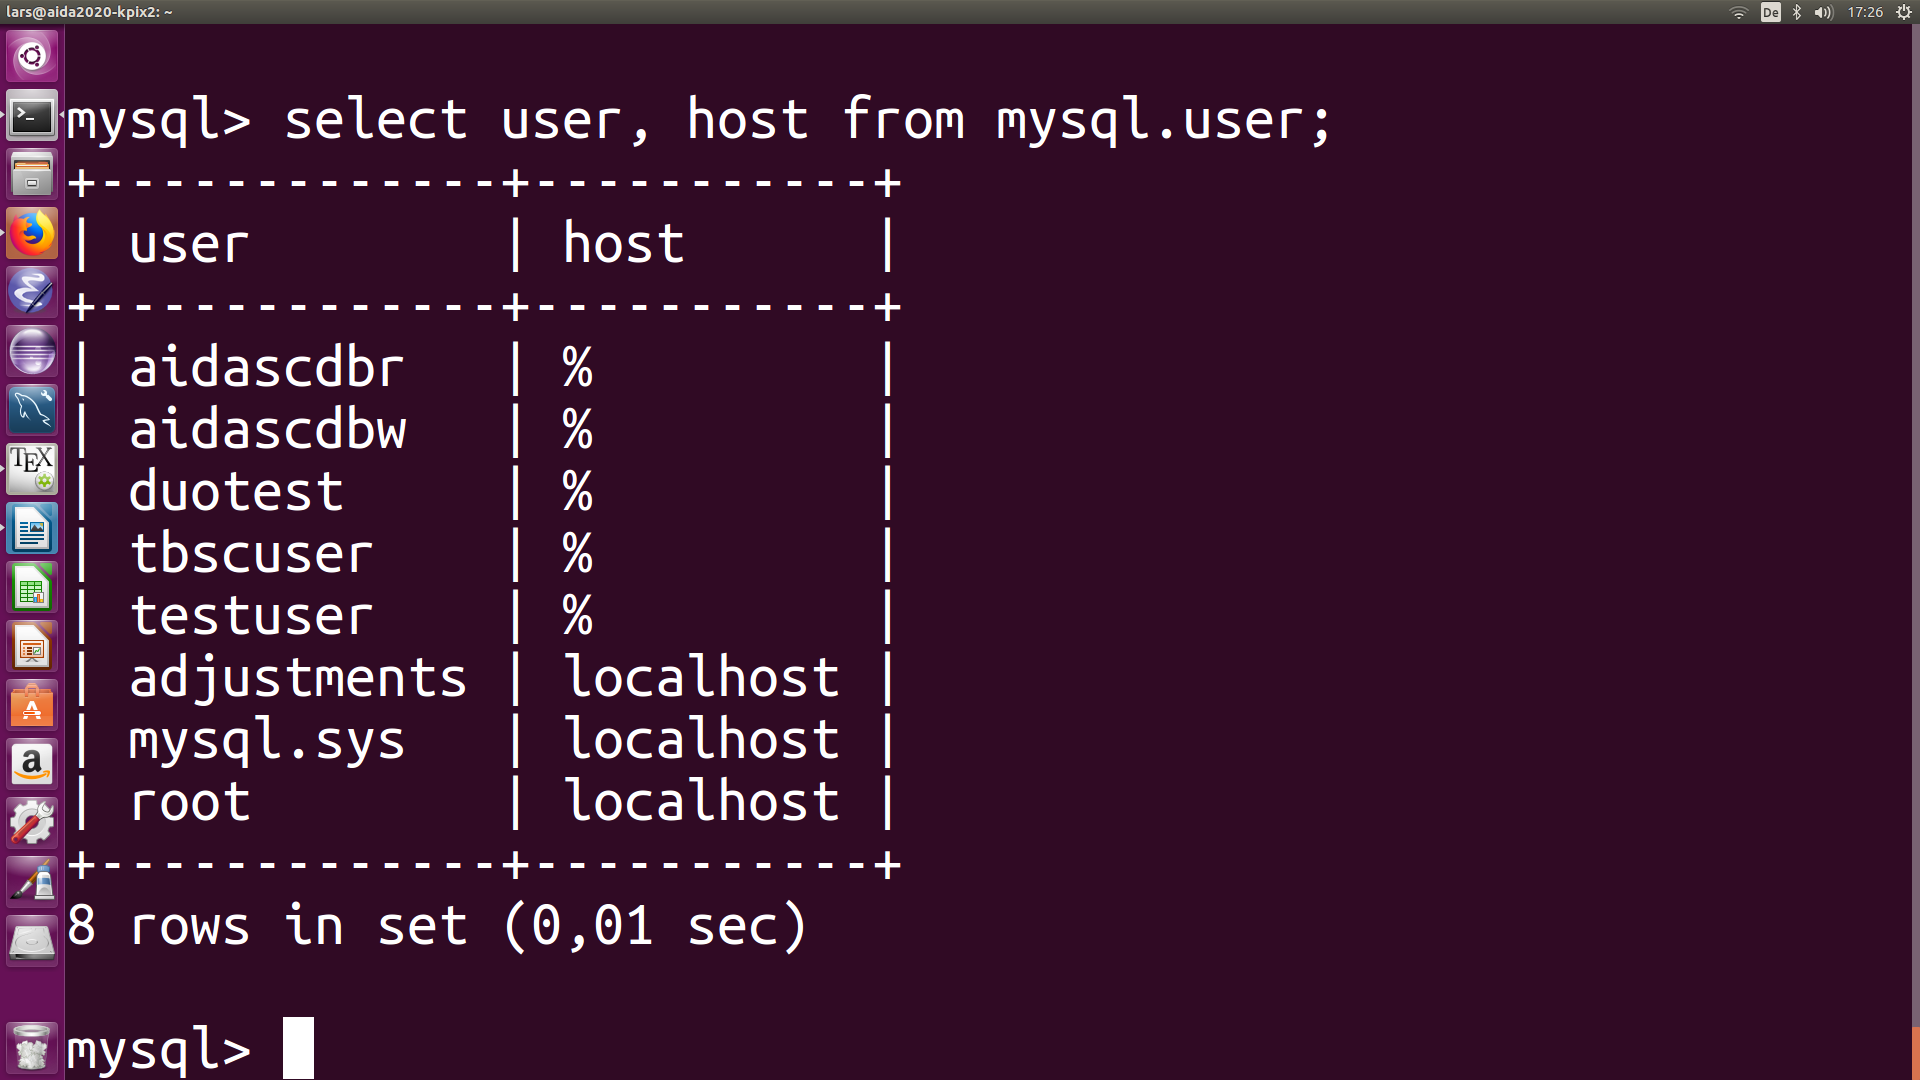
\includegraphics[trim={2cm 7cm 0cm 3cm},clip,width=0.65\textwidth]{figs/mysqluser.png}
\caption{Check the access rights of which hosts to all the users in the MySQL, in this case, \texttt{aidascdbr} represents the read-only user prepared for EUDAQ2, while \texttt{aidascdbw} represents the write-only user prepared for AMR.}
\label{fig:mysql-user}
\end{figure}

%If there is no \% behind the username (Fig. 4) you are using, either use a different user with remote access or create a new user with this access: \\
\textbf{Notice}: \texttt{\%} is used as wild character, to allow the relevant useraccount to be accessed from all different hosts; for a certain user, it may \texttt{GRANT} such \texttt{PRIVILEGES} for different host to access different DataBases/Tables; to check it, one can do (eg. \texttt{aidascdbw}):
\begin{lstlisting}[language=SQL]
mysql> SHOW GRANTS FOR 'aidascdbw'@'%';
+------------------------------------------------+
| Grants for aidascdbw@%                         |
+------------------------------------------------+
| GRANT ALL PRIVILEGES ON *.* TO 'aidascdbr'@'%' |
+------------------------------------------------+
\end{lstlisting}

\textbf{Currently}, all privileges given to MySQL users registered for AMR and for EUDAQ2, to access from any host (\verb|'aidascdbr'@'\%'|) to any database (\verb|*.*|); once the privileges needed for each is fixed, one should change this. For a current setup, one can use the following commands to give privileges:
%\colorbox{lightgray}{\texttt{mysql> GRANT ALL PRIVILEGES ON *.* TO 'USERNAME'@'\%' IDENTIFIED BY 'PASSWORD';}}\\
\begin{lstlisting}[language=SQL]
mysql> GRANT ALL PRIVILEGES ON *.* TO 'aidascdbr'@'\%' IDENTIFIED BY 'PASSWORD';
\end{lstlisting}

For creating a DataBase with tables, you can either log in any \texttt{USERNAME}, via which you want this database can be accessed;
or you can log in as the \verb|root| user, create the DataBase and later you \verb|GRANT PRIVILEGES| to some \verb|USERNAME|.
Here are the example commands to create a DataBase named `tbscs' with the a table named `tab\_rx':
\begin{lstlisting}[language=SQL]
mysql> CREATE DATABASE 'tbscs';
mysql> create table 'tab_rx' ('counter' int unsigned zerofill auto_increment, 'timer' datetime NOT NULL, 'temperature' double);
\end{lstlisting}

\subsection{ODBC}

This system is using the ODBC (Open DataBase Connectivity) in the Windows as interface between the AMRSoftware and the remote MySQL DataBase, and its 32bit version~\cite{odbc} is used due to compatibility which can be found in \verb|c:\Windows\SysWOW64\odbcad32.exe|.

In order to talk to MySQL, a driver for the ODBC is needed, see Ref~\cite{mysql-odbc}. \textbf{Notice:} this was already done, so if user has any problem relevant (e.g. different DataBase needed and etc.), please contact the system admin as only the administrator of the Windows PC is allowed to do this.

For each MySQL DataBase, it needs to be registered as a System Data Source Name (DSN) or User DSN for AMR to recognize. Here is an simple example to show how to add a new DSN, please notice, only administrator can add a system DSN, others can only add a user DSN. It is tested in Januaray 2018 with our first user experience, that AMR can work with a user DSN without any problem.

\begin{figure}[!ht]
\centering
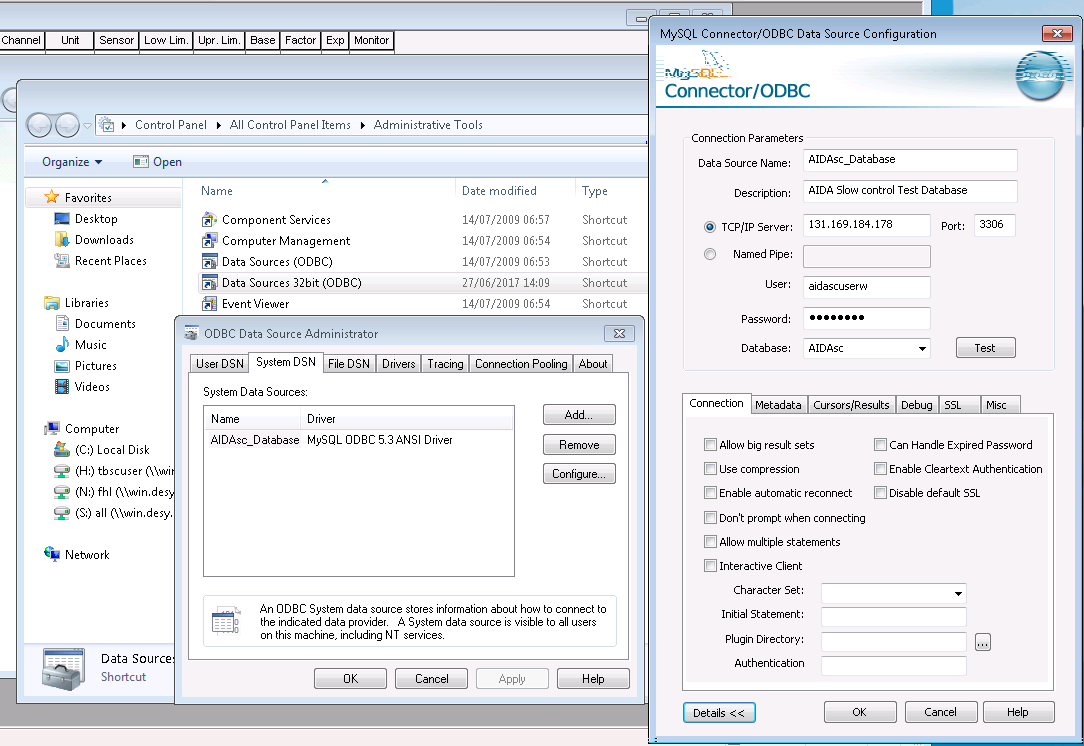
\includegraphics[width=0.8\textwidth]{figs/ODBC.png}
\caption{The windows one needs to open to register a new System/User DSN for connecting a MySQL DataBase to a Windows system via ODBC.}
\label{fig:dsn}
\end{figure}

The windows one needs to open to register a (user) DSN is shown in Figure~\ref{fig:dsn}:
\begin{itemize}
  \item Open the ODBC data source administrator: \verb|c:\Windows\SysWOW64\odbcad32.exe|;
  \item Click `Add' under the register User or System/User DSN, then choose the `MySQL' driver and continue with the configuration window (rightmost in Figure~\ref{fig:dsn}).
  \item Under the `MySQL Connector/ODBC Data Source Configuration' window: name your data source, give the correct TCP/IP address of the PC where the DataBase is located, Port is usually given as 3306, and put the User with its password to access the Database you are going to register. Please \textbf{notice} that you give this Windows PC access right to under this MySQL User to the DataBase you are going to use.
  \item Choose the target DataBase for transferring slow control data. To test if your connection is working or not, simply click on the `Test' button.
\end{itemize}

\subsection{AMR}
The AMRSoftware was installed under purchase form the ALMEMO company. If there is a problem encountered, please contact the local support group, and we can also get support by the company. If there is any new hardware added, please also contact the local support group for updating with the AMR software.

One needs to configure the AMR in terms of online export via ODBC, to do so, one simply needs to click \texttt{AutoSave} from the AMR Software window, then click \texttt{Add...} and choose \texttt{Add Online ODBC Export} as shown in Figure~\ref{fig:amr-conf1}~(left).
Also give one example to show how the DSN is added for AMR to talk with, and how to start it proper to transfer data.

\begin{figure}[!ht]
\centering
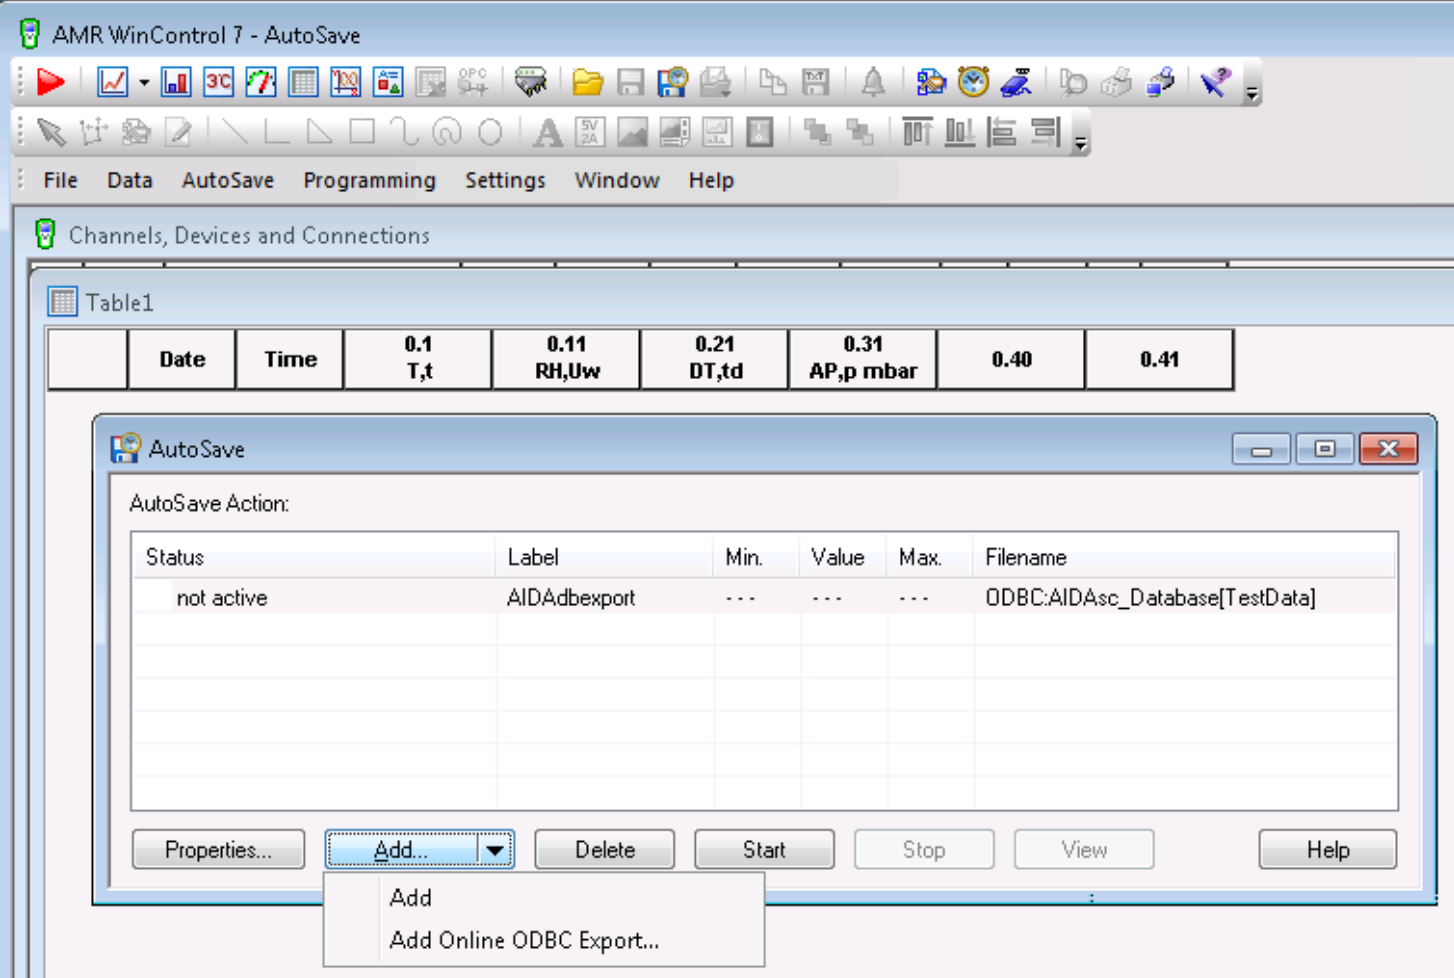
\includegraphics[height=12em]{figs/AMR_AutoSave.png}%
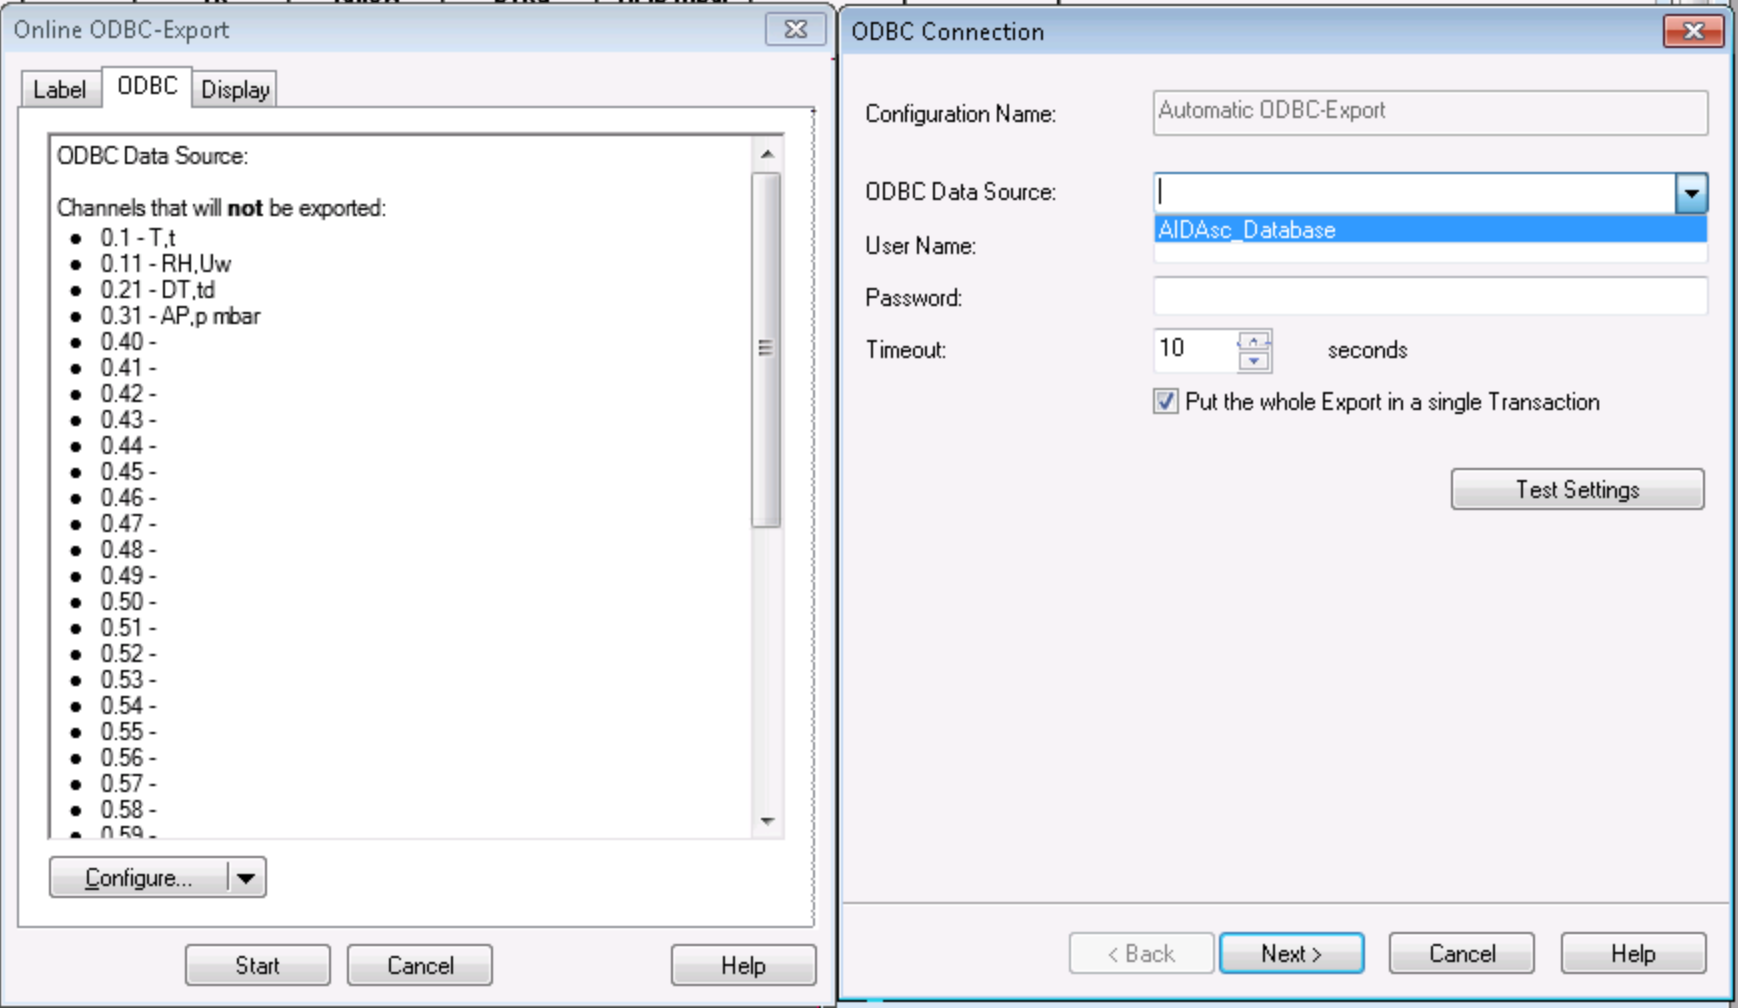
\includegraphics[height=12em]{figs/AMR_odbc.png}
\caption{Windows for adding an online ODBC Export entry to AMR software for exporting data out to a remote/local database via ODBC.}
\label{fig:amr-conf1}
\end{figure}

\subsection{unixODBC}
On the Linux PC where the EUDAQ2 is installed, a linux version of ODBC, namely unixODBC, is used. One can of course use the MySQL C++ connector library to connect MySQL DataBase with C++ code directly, but the point here is to provide a flexible scheme for this system to move to different SQL DataBase easily.

The unixODBC is not installed by default in linux, and it can be download from \href{http://www.unixodbc.org/}{http://www.unixodbc.org/}. A driver is also needed to connect to a MySQL DataBase, that can be downloaded from https://dev.mysql.com/downloads/connector/odbc/. Drivers are not automatically added to unixODBC, one also needs to configure it. All of the installation should be done already, in case of any change needed, please contact the system admin for administrator right to modify/change.

The unixODBC will be initialized everytime you login the system, using a init file \verb|/etc/odbcinst.ini|.
This file is already moved to \verb|/usr/local/etc| in order to provide access of the DSN to all the linux Users instead of admin only.
Therefore, please add the following line to your shell init file, such as \verb|.bashrc|:
\begin{lstlisting}[language=bash]
export ODBCSYSINI=/usr/local/etc
\end{lstlisting}

%There are two approaches to create/add a new DataBase connection to the system via unixODBC.
%The first way is to change the system file \verb|/etc/odbcinst.ini| then copy it again to the , and thus a System DSN can only be added by the Linux Users with the administrator right.
\subsubsection*{Add a DSN}
One can create a DSN template file, \verb|/usr/local/etc/odbc.ini|, as shown in Figure~\ref{fig:unixODBC} then install/register it to the system. An example to show how-to is followed:
\begin{enumerate}[label=(\roman*)]
  \item In the \verb|odbc.ini|, one needs to start a DSN with its name, as `odbcAidaSC' in Figure~\ref{fig:unixODBC}, then specify the DataBase, username with password, DataBase   server and unixODBC Driver. It is not of importance where the template file is stored.
  \item Once a \verb|odbc.ini| is newly added or updated, run the \verb|odbcinst| executable to register/update with the following command in the terminal~\cite{unixodbc-howto}:%[3]
  \begin{lstlisting}[language=bash]
$ odbcinst -i -s -f /usr/local/etc/odbc.ini\end{lstlisting}
  To check if the DSNs are added correctly to the system via unixODBC:
  \begin{lstlisting}[language=bash]
$ odbcinst -q -s
[odbcAidaSC]\end{lstlisting}
\end{enumerate}

\begin{figure}[!ht]
\centering
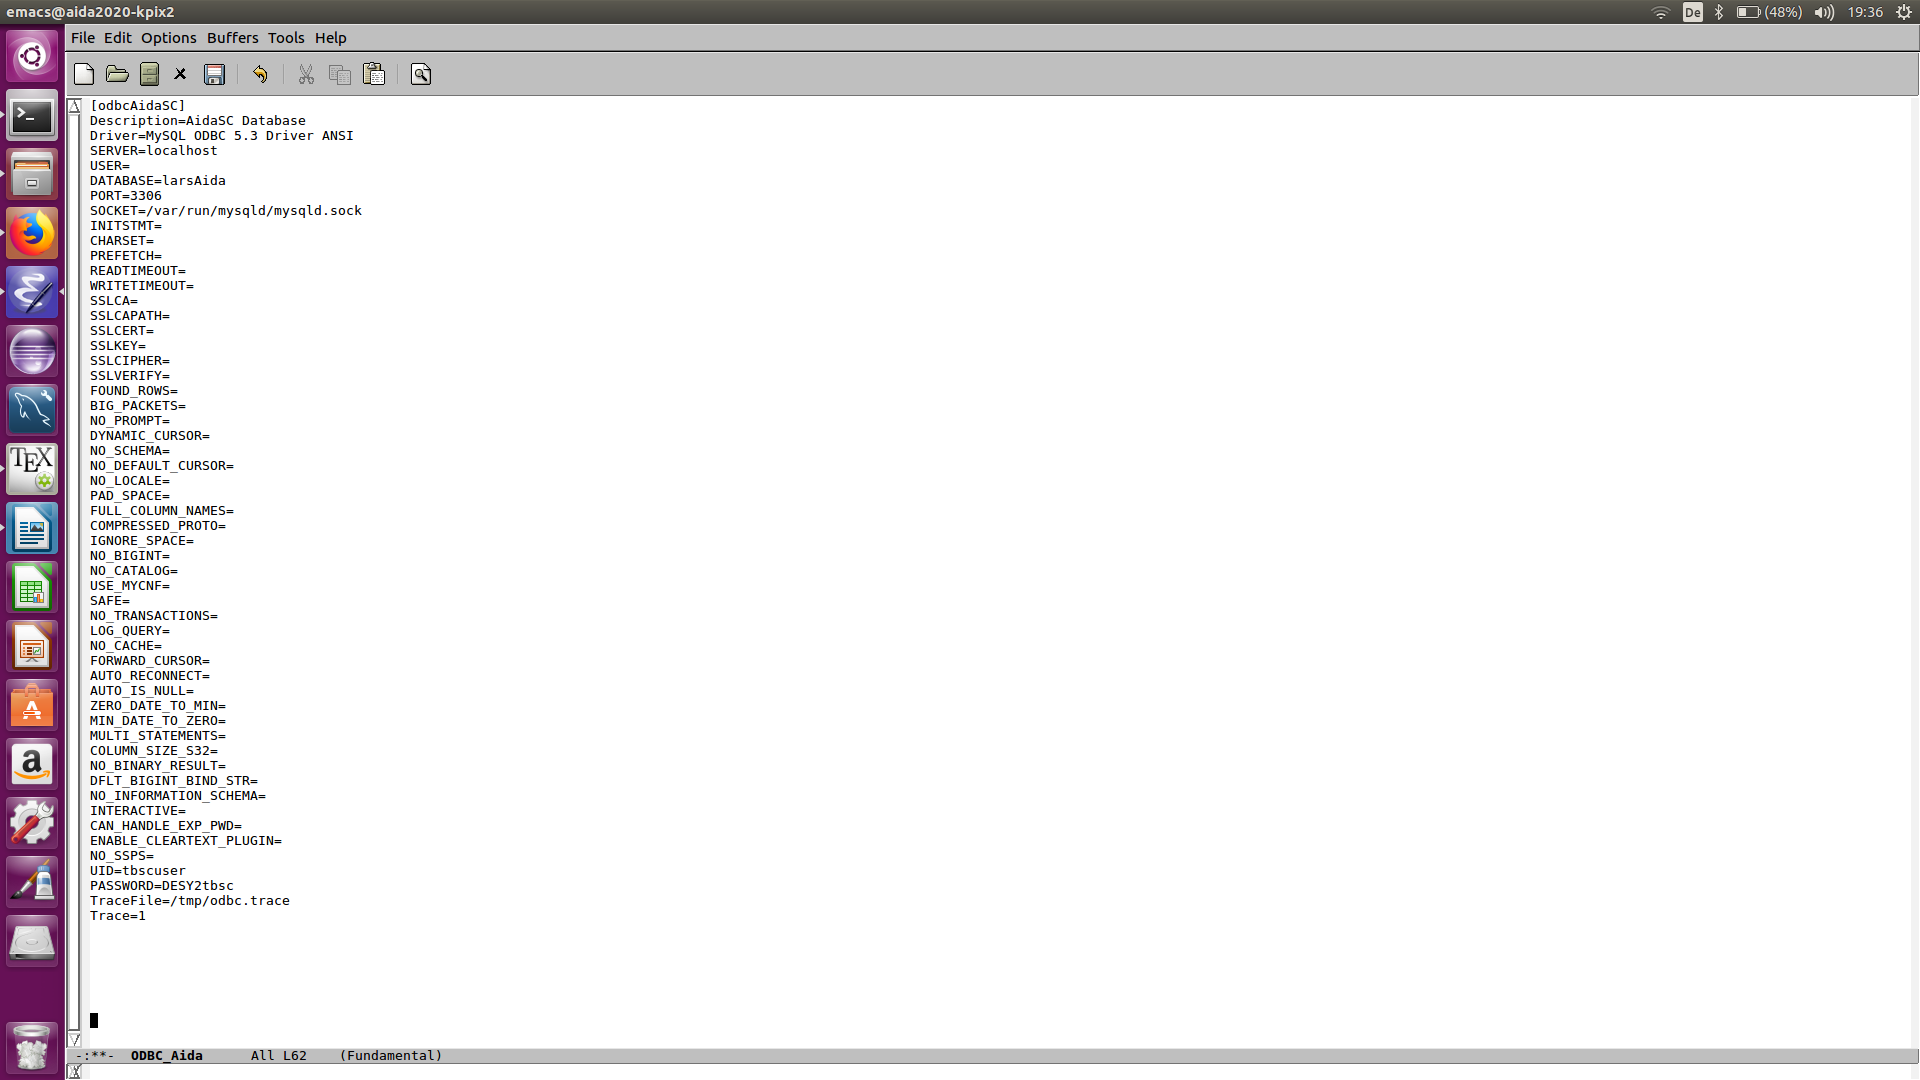
\includegraphics[trim={2.5cm 5cm 50cm 3.5cm},clip,width=7cm]{figs/unixtemplate.png}
\caption{An example of a unixODBC DSN template file: \texttt{odbc.ini}.}
\label{fig:unixODBC}
\end{figure}

\subsection{EUDAQ2}
The EUDAQ2~\cite{eudaq2} is the second version of the EUDAQ data acquisition framework, which is commonly used for many lively running Mimosa telescopes in the world. At DESY, there are two Mimosa telescopes, Duranta and Datura that are frequently demanded by users (~70\% users in 2017), and one AIDA2020 strip telescope under construction, all of which are using EUDAQ2 as the DAQ user interface.
Therefore, to unify the DAQ user interface for test beam users at DESY, this system is also designed based on the EUDAQ2 framework.

The EUDAQ2 software is usually provided and maintained by the local testbeam support group. In case of need, one can find simple instruction to download and install an EUDAQ locally from here: \href{http://eudaq.github.io}{http://eudaq.github.io}. \textbf{Notice:} please be sure that you have \verb|cmake| and \verb|cmake-qt-gui| installed to compile the code, if not, use \verb|sudo apt-get install| command to install them; a \texttt{Qt5} is also required to have the EUDAQ2 GUI produced, if not please download an open source version of the Qt Framework from their website: \href{https://www.qt.io}{https://www.qt.io}.

\textbf{Notice:} the EUDAQ2 modules for this sytem is not yet merged into the central master branch, for testbeam users, it should be already provided on the hut PC. In case that one needs to install on his/her own, please follow the following steps:
\begin{itemize}
  \item once you have the EUDAQ2 master branch installed from the central git repository, go to \verb|$EUDAQ2/user/| directory;
  \item clone the slow control modules here:
  \begin{lstlisting}[language=bash]
$ git clone https://github.com/DESY-TBSC/DESYtbsc.git \end{lstlisting}
  \item go to \verb|$EUDAQ2/build/| directory, do \verb|cmake-gui ..|, and make sure you have options with \texttt{USER\_TBSCDESY} all chosen under the \texttt{USER} category;
  \item compile it with all executables/librairies installed:
  \begin{lstlisting}[language=bash]
$ make install -j4  \end{lstlisting}
\end{itemize}

\section{How-to Take Data}
Once all the APIs and Softwares from Secion~\ref{sec:swsetup} are well installed and configured. To prepare for data taking: firstly one needs to make sure the data logger and the Windows PC on the rack are on, as well as the Linux PC where the MySQL and EUDAQ2 are installed is on; seconldy, both PCs need to connect to the internet with the same IP addresses as registered in the DSNs, and in the server/host access privileges given to the MySQL users. Any unexpected errors may arise if the system is not well configured/prepared. Before operating any data taking from the EUDAQ2 side, one needs to start the \texttt{polling} from the AMR system, and make sure that, in the AMR software, the \texttt{Online ODBC Export} entry under the \texttt{AutoSave} is `Start'.

Experience from the first user experience in January 2018 shows that the most common errors usually come from: wrong connections in the conf file and/or the AMR software is not polling and/or the ODBC export process is not `Start'.

Here below shows one step-by-step example, about how-to get slow control system data polled into your own EUDAQ2 data stream (integrated into your event as a tag):

\begin{enumerate}[label=(\roman*)]
  \item \textbf{Operate the AMR software}
  \begin{enumerate}
    \item remote log into the Windows PC on the rack using the \verb|xfreerdp|, e.g.:
    \begin{lstlisting}[language=bash]
xfreerdp /w:1600 /h:1000 /u:tbscuser /v:fhl-tb-sc01 /cert-ignore    \end{lstlisting}
    \item open the AMR software from the Desktop, as shown in Figure~\ref{fig:amr};
    \item verify the ODBC connection is active (in case the MySQL PC is not connected or configuration went wrong), by clicking `Test' in the `MySQL Connector/ODBC Data Source Configuratio' window, shown in bottom left in Figure~\ref{fig:amr};
    \item \textbf{START ODBC Transfer:} in the AMR software window, open \texttt{AutoSave}, choose the entry with `export' lablled, and click \texttt{Start};
    \item \textbf{START DATA POLLING:} click the RED arrow bottom on the top left of the AMR software window, see Figure~\ref{fig:amr}, to start the \texttt{Polling} process, and it will start blinking red and yellow when data is taken;
    \item \textbf{STOP DATA POLLING:} click the the same RED bottom to stop.
  \end{enumerate}
  \item \textbf{Start from EUDAQ2}
  \begin{enumerate}
    \item go to your EUDAQ2 directory \verb|cd $EUDAQ2|;
    \item to start the EUDAQ2 GUI:
    \begin{lstlisting}[language=bash]
cd bin/
./euRun    \end{lstlisting}
    \item to load the slow control modules, Producer to connect to the MySQL, and DataCollector to write data into a EUDAQ2 raw file:
    \begin{lstlisting}[language=bash]
./euCliProducer -n tbscProducer -t tbsc
./euCliCollector -n tbscDataCollector -t tbscDC    \end{lstlisting}
    \item all the loaded modules will be shown in the \texttt{Connections} panel, see Figure~\ref{fig:eudaq2_GUI}, then to load the init and config files, simply click `Load' button. Examples init/conf files are available in the directory of \verb|$EUDAQ2/user/tbscDESY/misc/|.
  \end{enumerate}
\end{enumerate}

\begin{figure}[!ht]
\centering
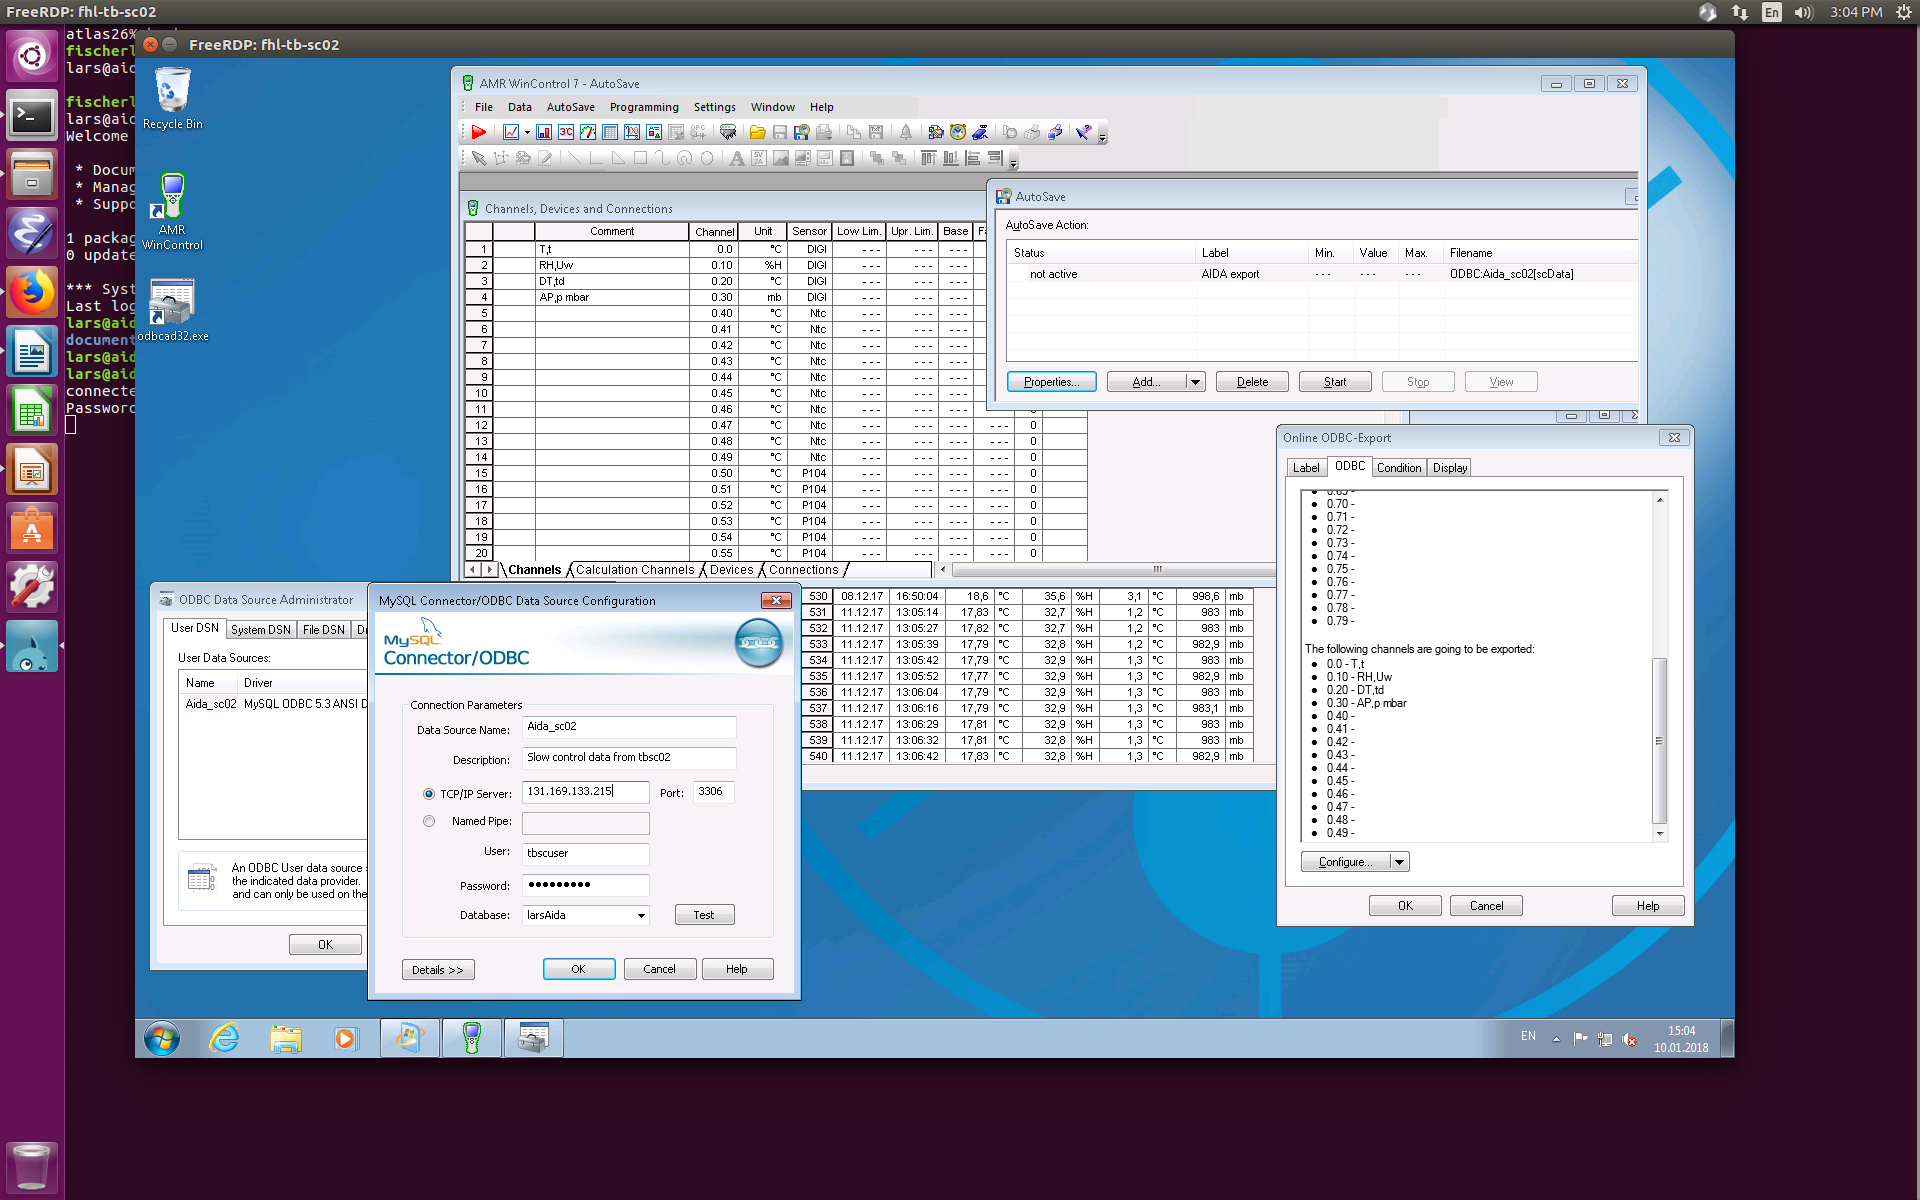
\includegraphics[trim={5cm 5cm 7cm 2cm},clip,width=0.85\textwidth]{figs/AMRSoftware.png}
\caption{The Windows OS from the rack PC via a xfreerdp, with opened windows of the AMR software (AMR WinControl7, top central) with its AutoSave configuration (right), and ODBC Data Source Adminitration with MySQL connector configuration (bottom left).}
\label{fig:amr}
\end{figure}

\begin{figure}[!ht]
\centering
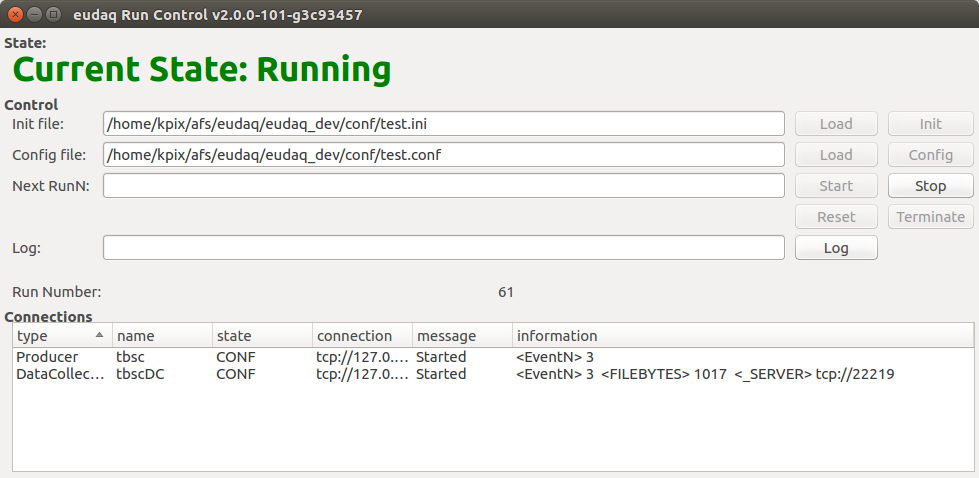
\includegraphics[width=0.8\textwidth]{figs/EUDAQ2_GUI_TBSC.png}
\caption{EUDAQ2 GUI example with slow control system modules loaded, example init and conf files loaded.}
\label{fig:eudaq2_GUI}
\end{figure}

\section{How-to display results}
An online monitor is currently under development, in collaboration with the DQM4Hep team, as a sub-task of integrating DQM4Hep to EUDAQ2.
Besides, two methods provided to display the slow control results after one data taking run:
\begin{itemize}
  \item Either one can use \verb|euCliReader| under the \verb|$EUDAQ2/bin/| directory, to readout all the events recorded in the \verb|.raw| output;
  \item Or one can use \verb|tbscCliConverter| under the \verb|$EUDAQ2/bin/| directory, to convert the slow control variables of all the events from the \verb|.raw| file to a \verb|.csv| file, see command example:
  \begin{lstlisting}[language=bash]
./tbscCliConverter -i tbsc02_180117123547_run000070.raw -o test_out.csv -ip
\end{lstlisting}
  The option \verb|-ip| is optional, it is to enable event printing during the converting process.
\end{itemize}

Histograms of temperature and humidity collected by different sensors on the rack are shown in Figure~\ref{fig:res-eg1}, based on data collected in testbeam area T24 at DESY. A nice agreement is expected to observe from data output from EUDAQ2 to data from MySQL databse dump, which validate the system stability.

\begin{figure}[!ht]
\centering
\includegraphics[width=0.45\textwidth]{figs/allTemperatures.pdf}%
\includegraphics[width=0.45\textwidth]{figs/HumiComp.pdf}
\caption{Histograms of temperatures (left) and humidity (right) collected by slow control system sensors in January 2018. The empty marks show data collected via EUDAQ2, and the filled marks come from MySQL data, expected agreement observed.}
\label{fig:res-eg1}
\end{figure}


\section{Integrate your own DataBase}
The current target is to integrate at least one user application to this system.
\begin{itemize}
  \item User can either integrate easily by writing a small script to send their data to any favored DataBase.
  \item To integrate a different structured DataBase from user's monitor to the EUDAQ2, users can either choose to do their own or contact the local support group for help. This process can be a quite quick (~1-2 workdays) development because of using the \texttt{unixODBC}.
\end{itemize}

An example may be given with a later update of this document, or one can check the developer manual:\\
\indent \href{https://cds.cern.ch/record/2284369/files/AIDA-2020-NOTE-2017-007.pdf}{\footnotesize{https://cds.cern.ch/record/2284369/files/AIDA-2020-NOTE-2017-007.pdf}}

\clearpage
%\bibliography{myref}
\begin{thebibliography}{1}
\bibitem{eudaq2} Wing, M. et al., {\em Development of run control ready}, AIDA2020, AIDA-2020-MS62, \href{http://cds.cern.ch/record/2276456}{http://cds.cern.ch/record/2276456}
\bibitem{mysql-odbc} \href{https://dev.mysql.com/downloads/connector/odbc/}{https://dev.mysql.com/downloads/connector/odbc/}
\bibitem{unixodbc-howto} \href{https://manpages.ubuntu.com/manpages/xenial/man1/odbcinst.1.html}{https://manpages.ubuntu.com/manpages/xenial/man1/odbcinst.1.html}
\bibitem{odbc} \href{https://docs.microsoft.com/en-us/sql/odbc/microsoft-open-database-connectivity-odbc?view=sql-server-2017}{https://docs.microsoft.com/en-us/sql/odbc/microsoft-open-database-connectivity-odbc?view=sql-server-2017}
%% \bibitem{atlas-2l2v-int} ATLAS, ATL-COM-PHYS-2014-270 {\em Search for a Higgs boson in the $H\to ZZ \to \ell\ell\nu\nu$ Channel} 05 May 2015.
%% %\bibitem{atlas-2l2v-int} ATLAS \href{https://cds.cern.ch/record/1453770}{\em Signal studies in H to gamma gamma search with 8TeV data} 04 Jun 2012.
%% %% %% \bibitem{impj}  The Japan Reader {\em Imperial Japan 1800-1945} 1973: Random House, N.Y.
%% %% %% \bibitem{norman} E. H. Norman {\em Japan's emergence as a modern state} 1940: International Secretariat, Institute of Pacific
%% %% %%   Relations.
%% %% %% \bibitem{fo} Bob Tadashi Wakabayashi {\em Anti-Foreignism and Western Learning in Early-Modern Japan} 1986: Harvard University Press.

\end{thebibliography}

%1: https://dev.mysql.com/downloads/connector/odbc/ \\

\end{document}
